\section{LCD}
\subsection{Funktionsweise}

\begin{figure}[t]
  \centering
  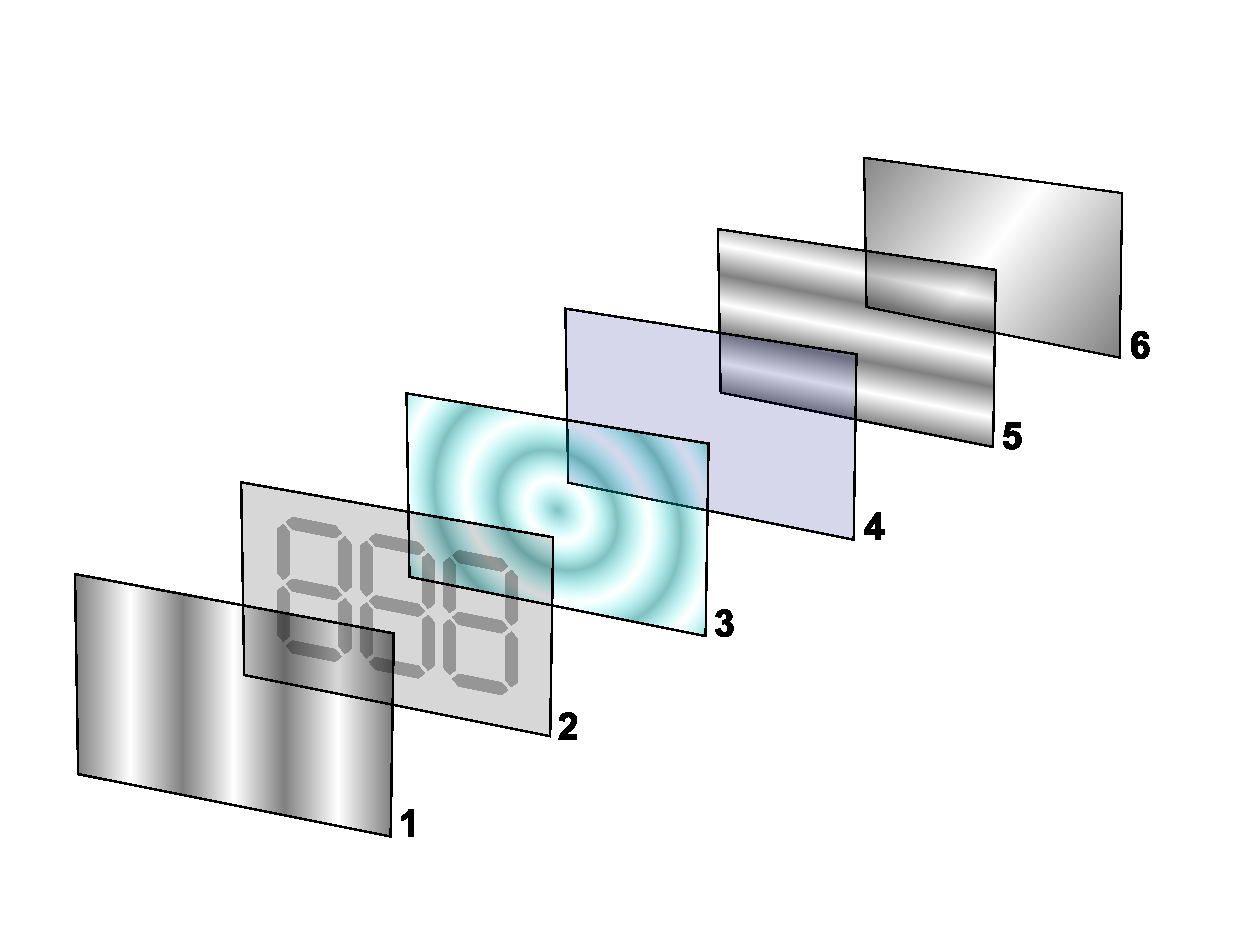
\includegraphics[width=\linewidth, keepaspectratio]{Bilder/LCD_layers}
  \caption{Aufbau eines LCDs mit Polarisationsfolien (Markierung 1 und 5), zwei beschichteten, leitenden Glasplatten (Markierung 2 und 4), den Flüssigkristallen (Markierung 3) und einem Reflektor (Markierung 6) nach ref[FIXME REF]}
  \label{lcdaufbau}
\end{figure}

Das Display besteht aus zwei zusammengeklebten Glasplatten mit einem Abstand von circa 10 Mikrometer. Auf den Glasplatten befinden sich leitende Schichten aus Indium-Zinn-Oxid. Diese Schichten werden später zur Darstellung von Zeichen verwendet. Grundsätzlicher Aufbau eines LCD Displays besteht aus folgenden Teilen (siehe Abbildung \ref{lcdaufbau}):
\begin{itemize}
\item zwei Glasplatten, die sich gegenüber liegende Innenseiten jeweils mit leitender Schicht bezogen (Markierung 2 und 4)
\item zwischen den Glasplatten: Flüssigkristall (Markierung 3)
\item außerhalb der Glasplatten: Polarisationsfolien (Markierung 1 und 5)
\item Ein Refelektor am Ende (Markierung 6)
\end{itemize}
Die Glasplatten werden so präpariert, dass die zigarrenförmige Moleküle auf jeweils einer Glasplatte in eine Richtung zeigen, auf der gegenüberliegenden Seite sind sie um 90 Grad gedreht. Flüssigkristall beschreibt somit eine “Schraubenstruktur”. Diese verschraubte Struktur veranlasst polarisiertes Licht, ihr zu folgen. Ohne Spannung wird Polarisationsebene um 90 Grad gedreht  und das Licht wird durchgelassen. Beim Anlegen von Spannung (ca. 3V Wechselspannung -> siehe Kapitel \ref{sec:elektronik}): Moleküle richten sich kollektiv senkrecht zu Elektroden aus, also existiert für das Polarisationslicht somit keine Schraubenstruktur mehr. Folglich wird beim Durchgang durch die Zelle der Polarisationszustand nicht beeinflusst, was schließlich dazu führt, dass die Bereiche dunkel erscheinen (Quellen: Bauanleitung und https://www.cmb-systeme.de/technikwissen/aufbau-und-funktion-einer-lcd-zelle)

\subsection{Produktionsschritte}
Schritt 1: Strukturierung der Elektroden, um Bereich, die leuchten sollen, abzudecken.\\
Schritt 2: Wegätzen der beschichteten Bereiche, die nicht leuchten sollen (mit 3-5\% Salzsäure), sodass die braune Färbung der Glasplatten verschwindet.\\
Schritt 3: Entfernen der Abdeckschicht (Klebefolie, siehe Abschnitt \ref{subsec:klebefolie}), dabei werden Klebereste mit Aceton entfernt.\\
Schritt 4: Oxidieren der Indium-Zinn-Schicht (im Ofen bei 300 Grad), damit die Glasplatten soweit wie möglich transparent erscheinen.\\
Schritt 5: Reinigung der Glasplatten durch das Kochen dieser in einem im Verhältnis 1:5 verdünnten alkalischen tensidfreien Reinigungsbad 3 bis 5 Minuten, damit die Glasplatten komplett fettfrei werden. Dabei werden auch Siedesteinchen verwendet, um einen Siedeverzug zu vermeiden.\\
Schritt 6: Orientierung der Glasoberfläche durch sogenanntes {\quote Reiborientieren}. Dabei wird je eine Oberfläche mit einem Zellstofftuch in eine bestimmte Richtung gerieben, sodass beide Oberflächen jeweils senkrecht zueinander ausgerichtet sind. \\
Schritt 7: Zwischen den Glasplatten werden Abstandshalter (am Rand) eingelegt, damit diese sich später mit einem Abstand von ca. 10 bis 15 Mikrometer  gegenüberliegen. Hier einigt sich Folie von z.B. Zigarettenschachteln, weil diese eine Dicke von ca. 12 Mikrometer aufweist.\\
Schritt 8: Die Glasplatten werden mit den Abstandshaltern übereinandergelegt. Dabei sollen sich die leitenden Seiten der Glasplatten gegenüberliegen. Danach werden zunächst sich zwei gegenüberliegenden Seiten der Glasplatten mit einem Zweikomponent-Kleber verklebt. Hierbei sollen die Glasplatten im Bereich der Abstandshalter zusammengepresst werden, um den Abstand zu bewahren, ansonsten zeigt die Zelle später eine langsamere elektrooptische Reaktion. \\
Schritt 9: An einer der noch offenen Seiten wird nun der Flüssigkristall durch Kapillarwirkung eingefüllt. Es werden Tropfen des  Flüssigkristalls an die noch offene Kanten gesetzt, und der Flüssigkristall zieht selber in die Zelle ein. Anschließend werden die noch offenen Kanten mit dem Kleber verschlossen.	
(Quelle: Bauanleitung)

\subsection{Elektrodenstrukturaufbringung}
\subsubsection*{Fotolack}
\subsubsection*{Klebefolie}\label{subsec:klebefolie}
Muster werden entworfen und mit einem Plotter aus einer selbstklebenden Klebefolie ausgeschnitten. Das Muster wird auf einer Übertragungsfolie aufgebracht und auf die leitende Schicht der Glasplatten aufgeklebt, anschließend wird die Übertragungsfolie abgezogen. Nun sind alle Stellen, die später leuchten sollen, abgedeckt.
\subsubsection*{Edding/Tesa}
Eine weitere Möglichkeit, die später zu leuchtende Stellen abzudecken, ist mit Hilfe von Tesa oder durch das direkte Aufmalen von Strukturen mit einem wasserfesten Edding. Diese Verfahren sind zwar einfacher, allerdings entstehen hierbei keine so scharfen Kanten wie durch eine Folie.
\subsection{Ätzen der Struktur}
\subsubsection*{Salzsäure}
\subsection*{Platinenätzmittel}
Das Wegätzen der Indium-Zinn Schicht ist auch durch das Ätzbad möglich, welches im FAUFabLab zum Ätzen von Platinen verwendet wird. Dazu wird eine Natriumpersulfatlösung verwendet und nach ca. 20 Minuten war bei unserem Versuch die leitende Indium-Zinn-Schicht entfernt. Diese Methode stellt also eine gute Alternatie zur Salzsäure dar.

\begin{figure}[t]
  \centering
  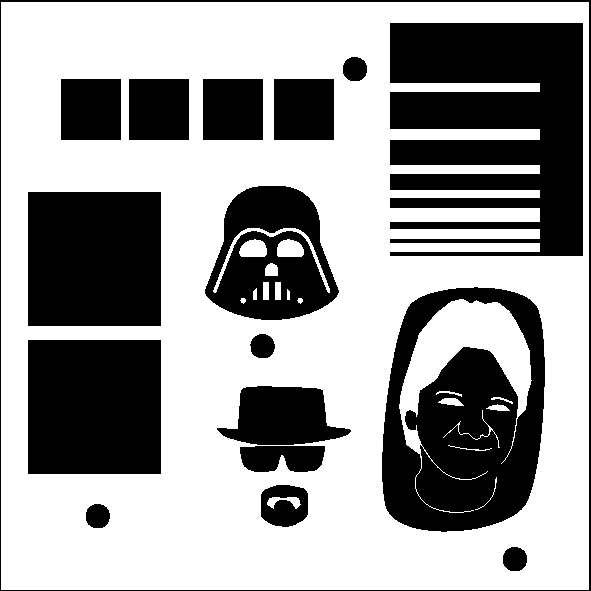
\includegraphics[width=\linewidth, keepaspectratio]{Bilder/testmuster}
  \caption{Testmuster (Anzeigen und Ausrichtungspunkte)}
  \label{testmuster}
\end{figure}

\begin{figure}[t]
  \centering
  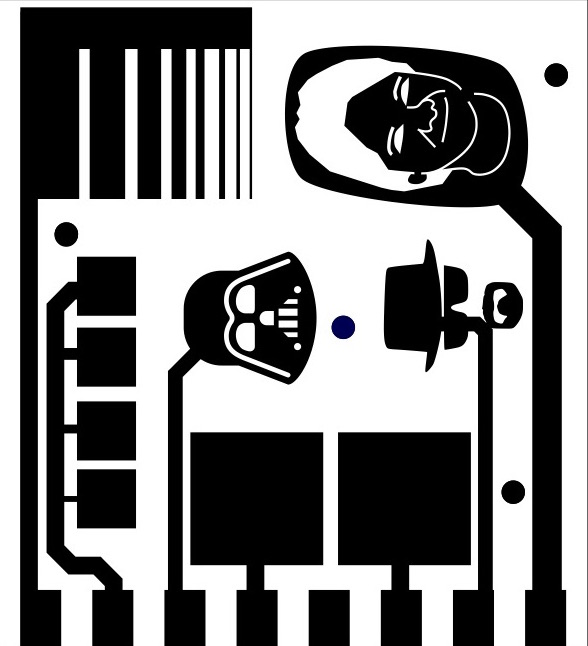
\includegraphics[width=\linewidth, keepaspectratio]{Bilder/testmuster-seite1}
  \caption{Testmuster (Anzeigen, Ausrichtungspunkte und Zuleitungen untere Seite)}
  \label{testmuster-seite1}
\end{figure}

\begin{figure}[t]
  \centering
  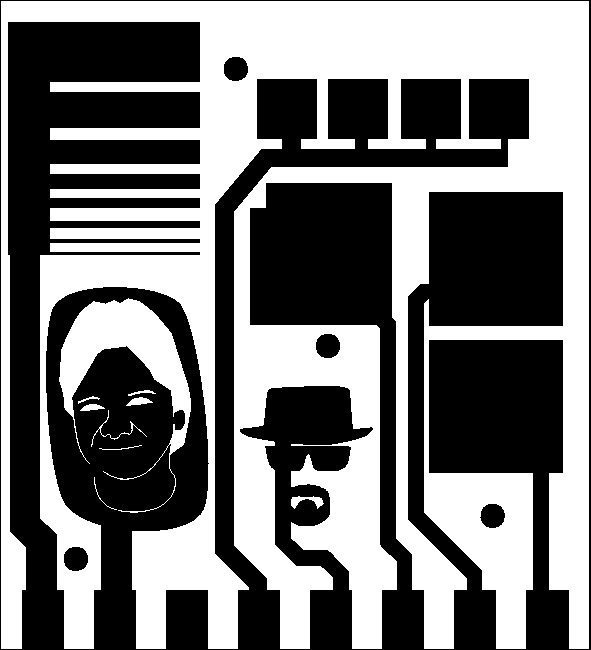
\includegraphics[width=\linewidth, keepaspectratio]{Bilder/testmuster-seite2}
  \caption{Testmuster (Anzeigen, Ausrichtungspunkte und Zuleitungen obere Seite)}
  \label{testmuster-seite2}
\end{figure}

\subsection{Oxidierung der Glasplatten}

Die Oxidierung der Indium-Zinn Schicht der Glasplatten zu Indium-Zinn-Oxid kann auf mehrere Arten erreicht werden. Im Folgenden werden die Verfahren forgestellt und deren Einsetzbarkeit abgewogen.
Indikatoren für eine gelungene Oxidierung sind:
\begin{itemize}
\item Die für die leitende Schicht typische brauen Färbung muss merklich verschwinden
\item Eine Messung mittels eines Multimeters muss eine Nennenswerte Änderung der Leitfähigkeit ergeben
\end{itemize}

\subsubsection{Wasserstoffperoxid}

Die Testplatte wurden in ein Wasserstoffperoxid-Bad gegeben und nach 1h wieder entnommen. Beide oben genannten Indikatoren haben nicht angesprochen, was darauf schließen lässt, dass der Oxidierungsversuch nicht erfolgreich war.
Nun soll ein Langzeittest über mehrere Tage Erkentnisse geben, ob der Oxidierungsvorgang bei einer längeren Einwirkungsdauer funktioniert. Dies war nicht der Fall.

Somit lässt sich festhalten, dass eine Oxidierung mittels Wasserstoffperoxid bei Raumtemperatur nicht möglich ist.

\subsubsection{Wasserstoffperoxid mit Hitze}

Da die Oxidierung bei Raumtemperatur nicht funktioniert hat wurde ein Versuch gestartet, die Indium-Zinn Schicht in erwärmten Wasserstoffperoxid durchzuführen.
Keiner der oben genannten Indikatoren wies auf eine Oxidierung hin, weshalb das Verfahren ebenfalls als nicht tauglich eingestuft werden kann.

\subsubsection{Hitze im Ofen}

Ein funktionierendes, aber sehr zeitaufwändiges, Verfahren ist die Oxidierung in einm Ofen. Hierbei kann ein gewöhnlicher Pizzaofen eingesetzt werden. Wir haben den Reflow-Ofen aus dem Fablab hierfür benutzt.
Bei einer Temperatur werden die Glasplatten mit der beschichteten Seite nach oben auf das Gitter gelegt. Wichtig ist, dass der Ofen maximal leicht vorgeheizt wurde, da zu starke Temperaturunterschiede die Glasplatten zum brechen bringen könnten. Nun wurden die Testplatten für 1:30h im Ofen belassen und anschließend für 30min abkühlen lassen.
Beide Indikatoren haben angeschlagen was zeigt, dass die Oxidierung erfolgreich war.

Da dies das einzig funktionierende Verfahren ist, wird es zur Herstellung der Displays eingesetzt.

\subsection{Ausrichtung der Glasplatten}
\subsection{Verkleben und befüllen}
2-K Kleber, Abstandhalter, Einfüllen des LCD
\subsection{Anzeigefähigkeit}
Selbst die kleinste Zuleitung (Dicke 1mm) bei den kleinen Rechtecken versorgt diese sicher mit Spannung und sie können somit angezeigt werden. Die kleinste Struktur beim Strukturtest wird ohne Probleme angezeigt (Dicke 0,4mm). Der Grund dafür sind die scharfen Kanten, die durch den Folienplott erreicht werden können. Die Ausrichtung ist gut möglich, da die Struktur nach der Oxidierung der Glasplatten noch leicht, aber dennoch gut sichtbar ist. Komplexe Strukturen (Walter White, Darth Vader, Jürgen) können ebenso ohne Probleme angezeigt werden. Vermutlich könnten diese noch verkleinert werden und dennoch ohne Probleme angezeigt werden.

\begin{figure}[]
    \centering
    %\subfigure[Caption]{   
       % 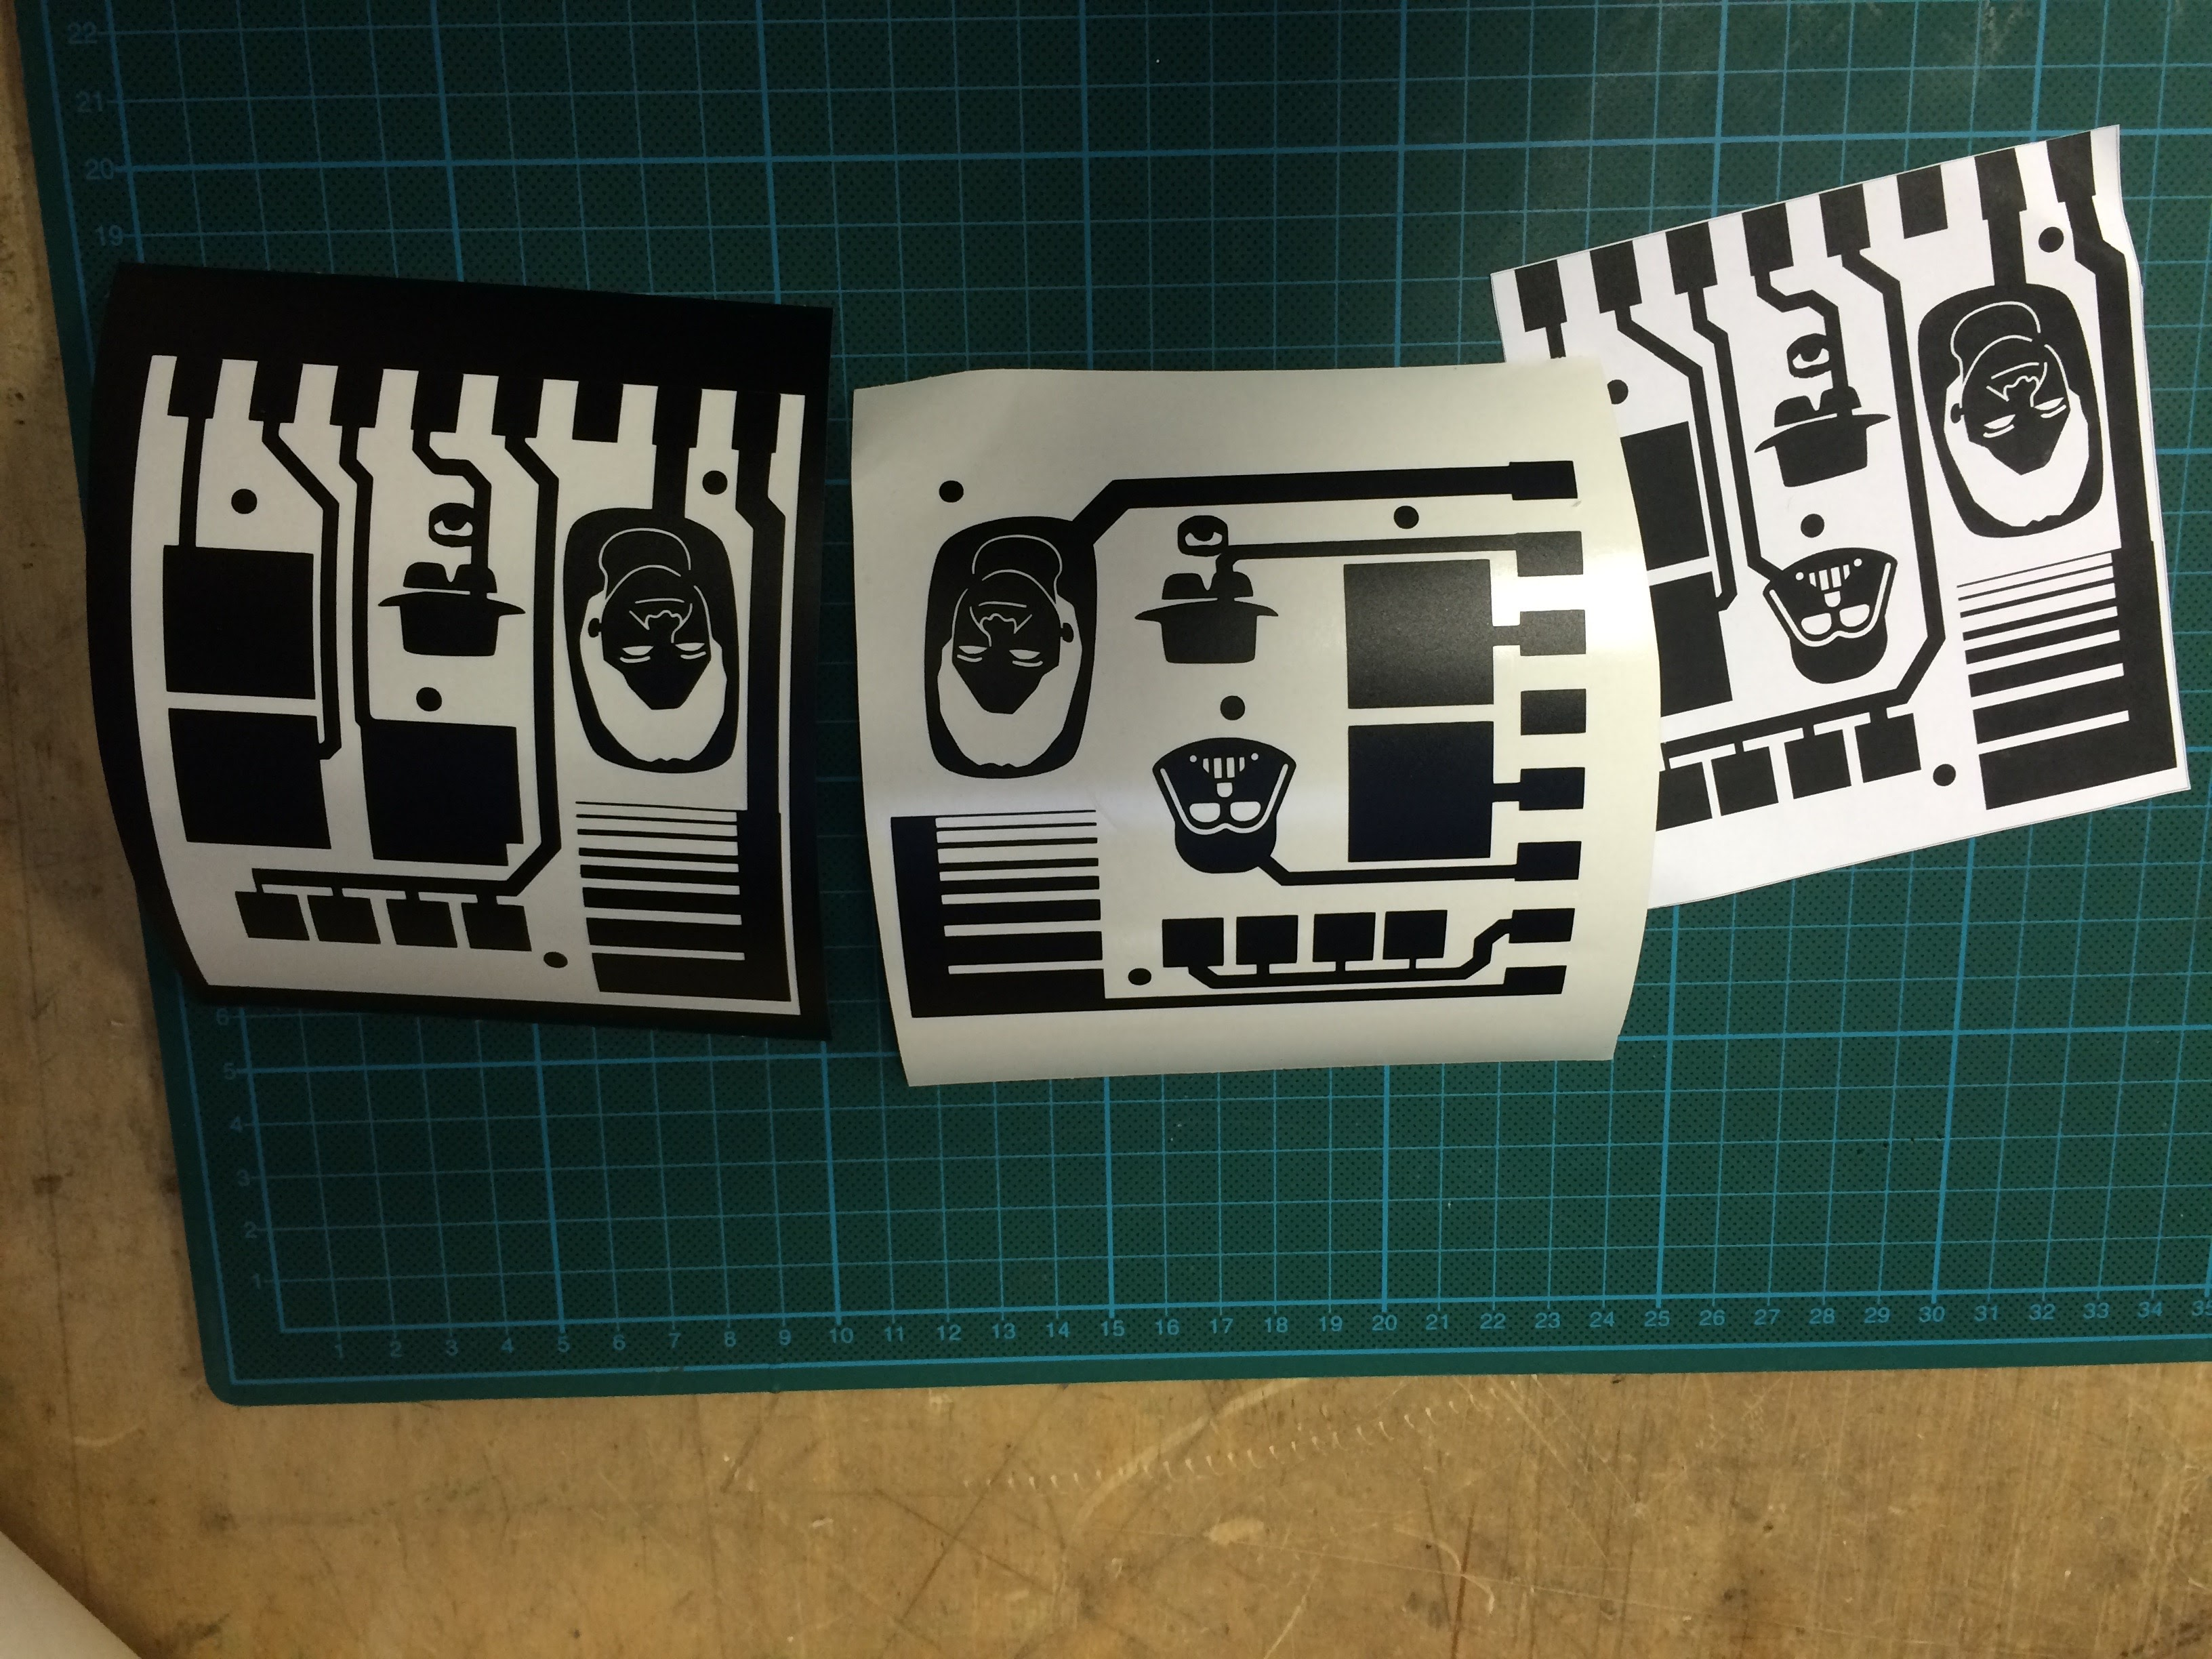
\includegraphics[width=0.22\textwidth]{./Bilder/Folie.jpg}
    %}
    %~ 
    \subfigure[Aufbringen der Klebefolie]{  
        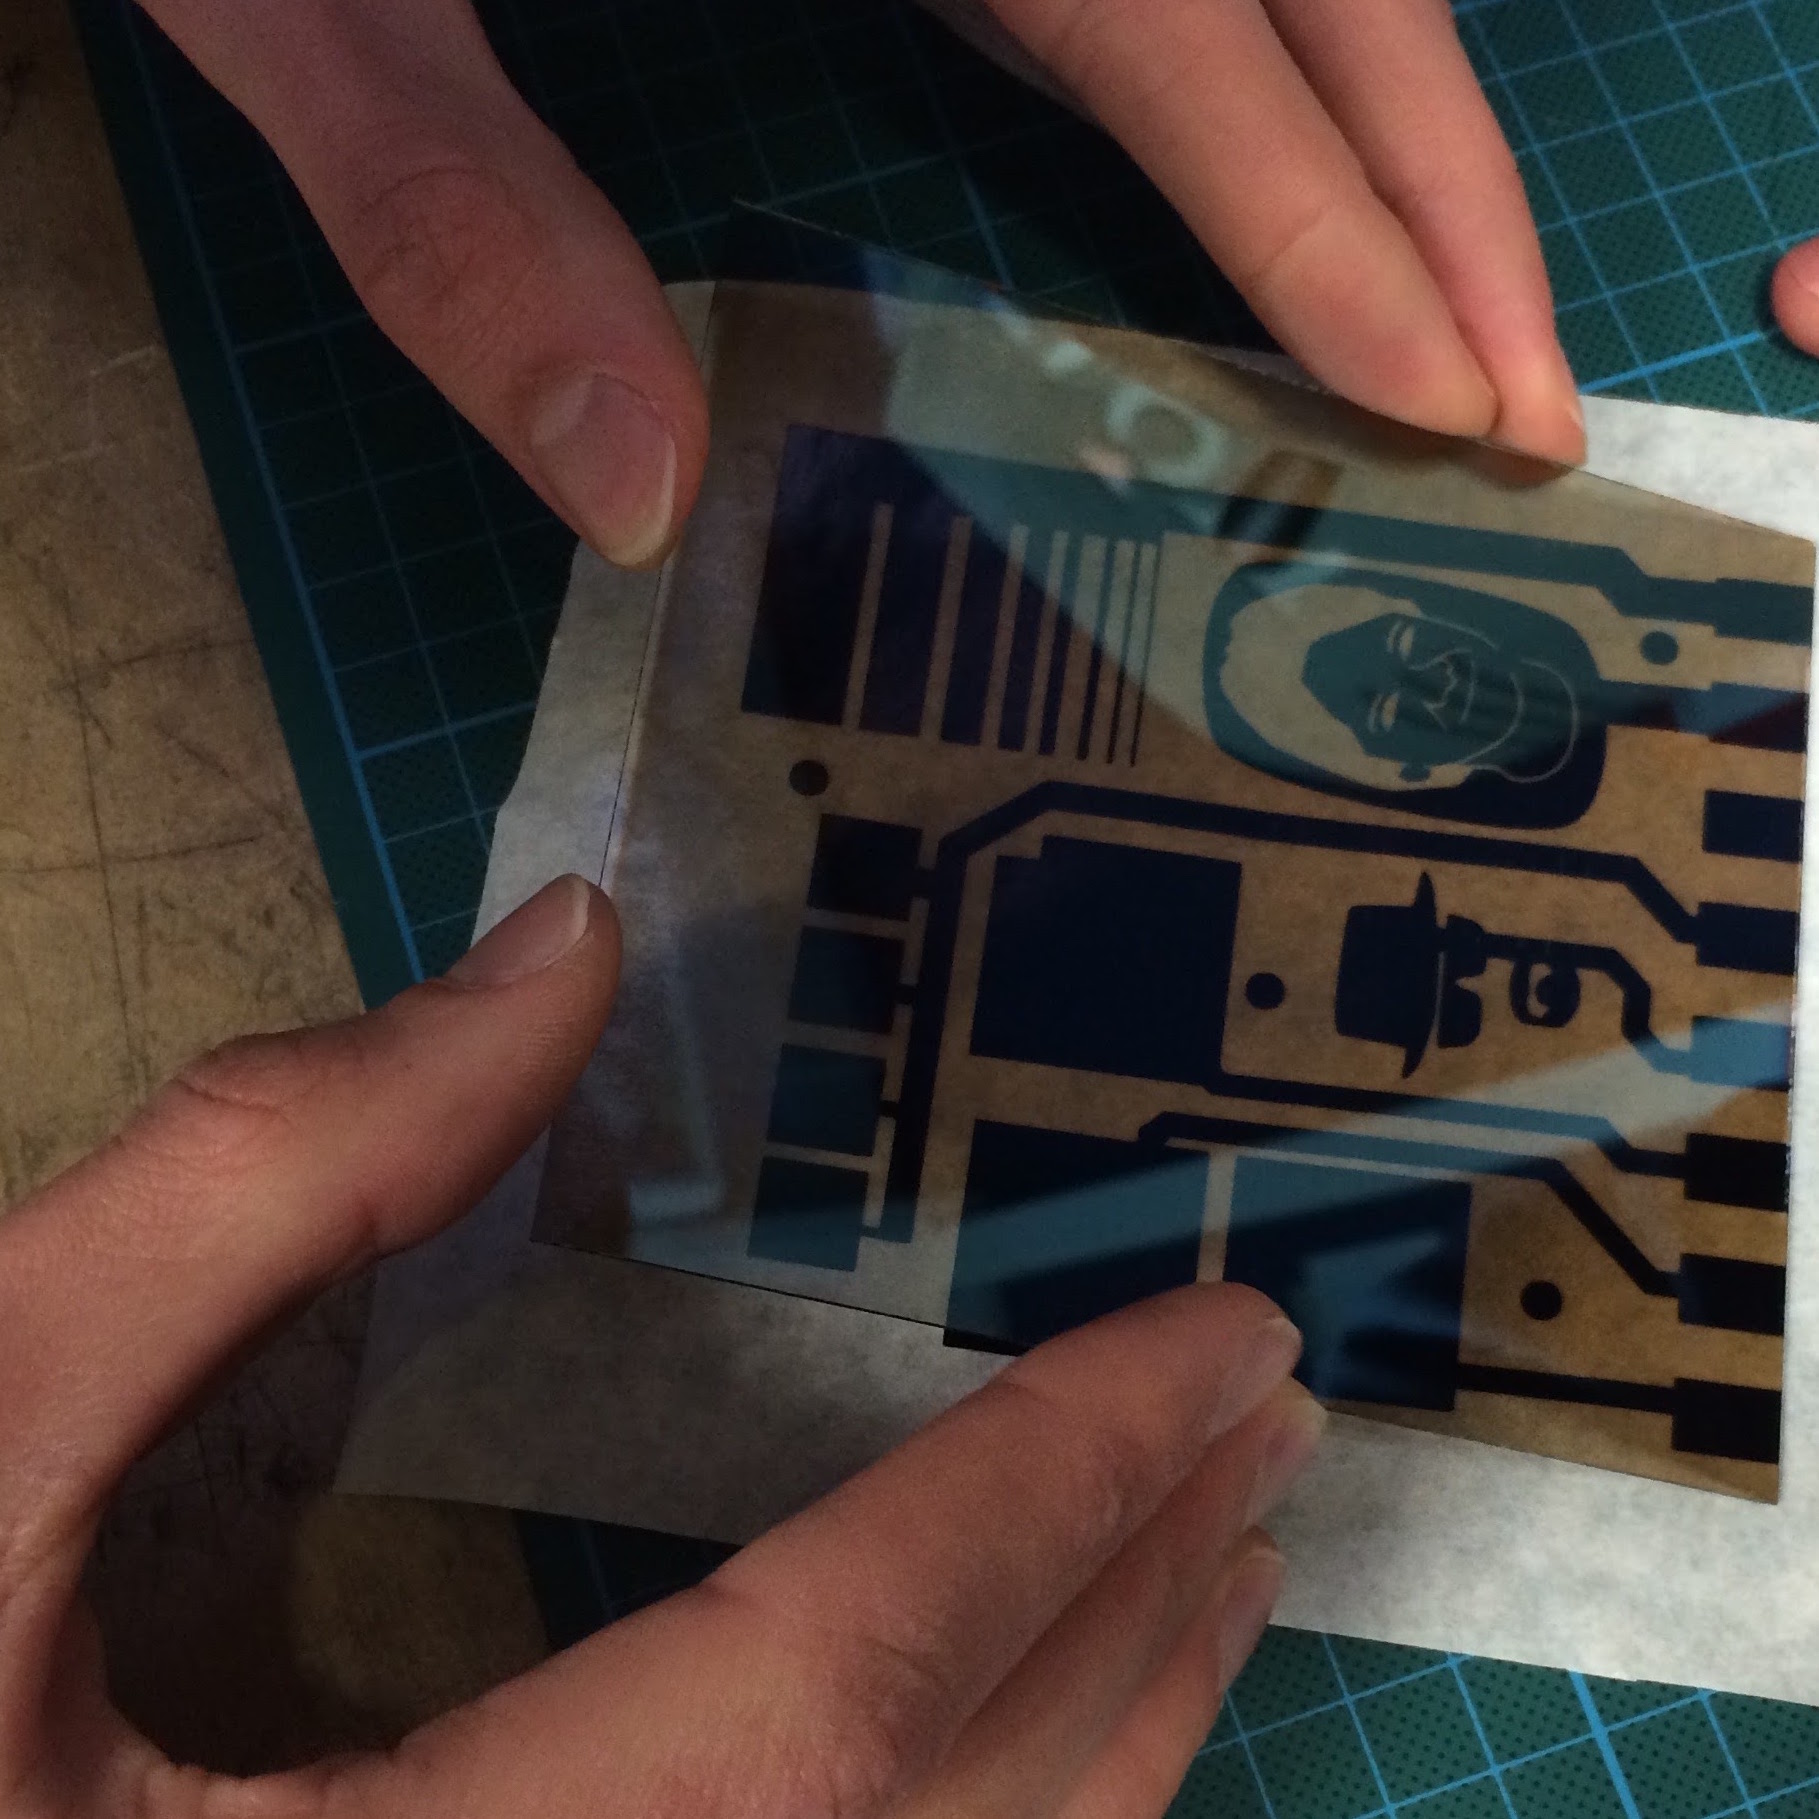
\includegraphics[width=0.22\textwidth]{./Bilder/Schritt1.jpg}    
    }
    ~
    \subfigure[Folie abziehen]{	
   		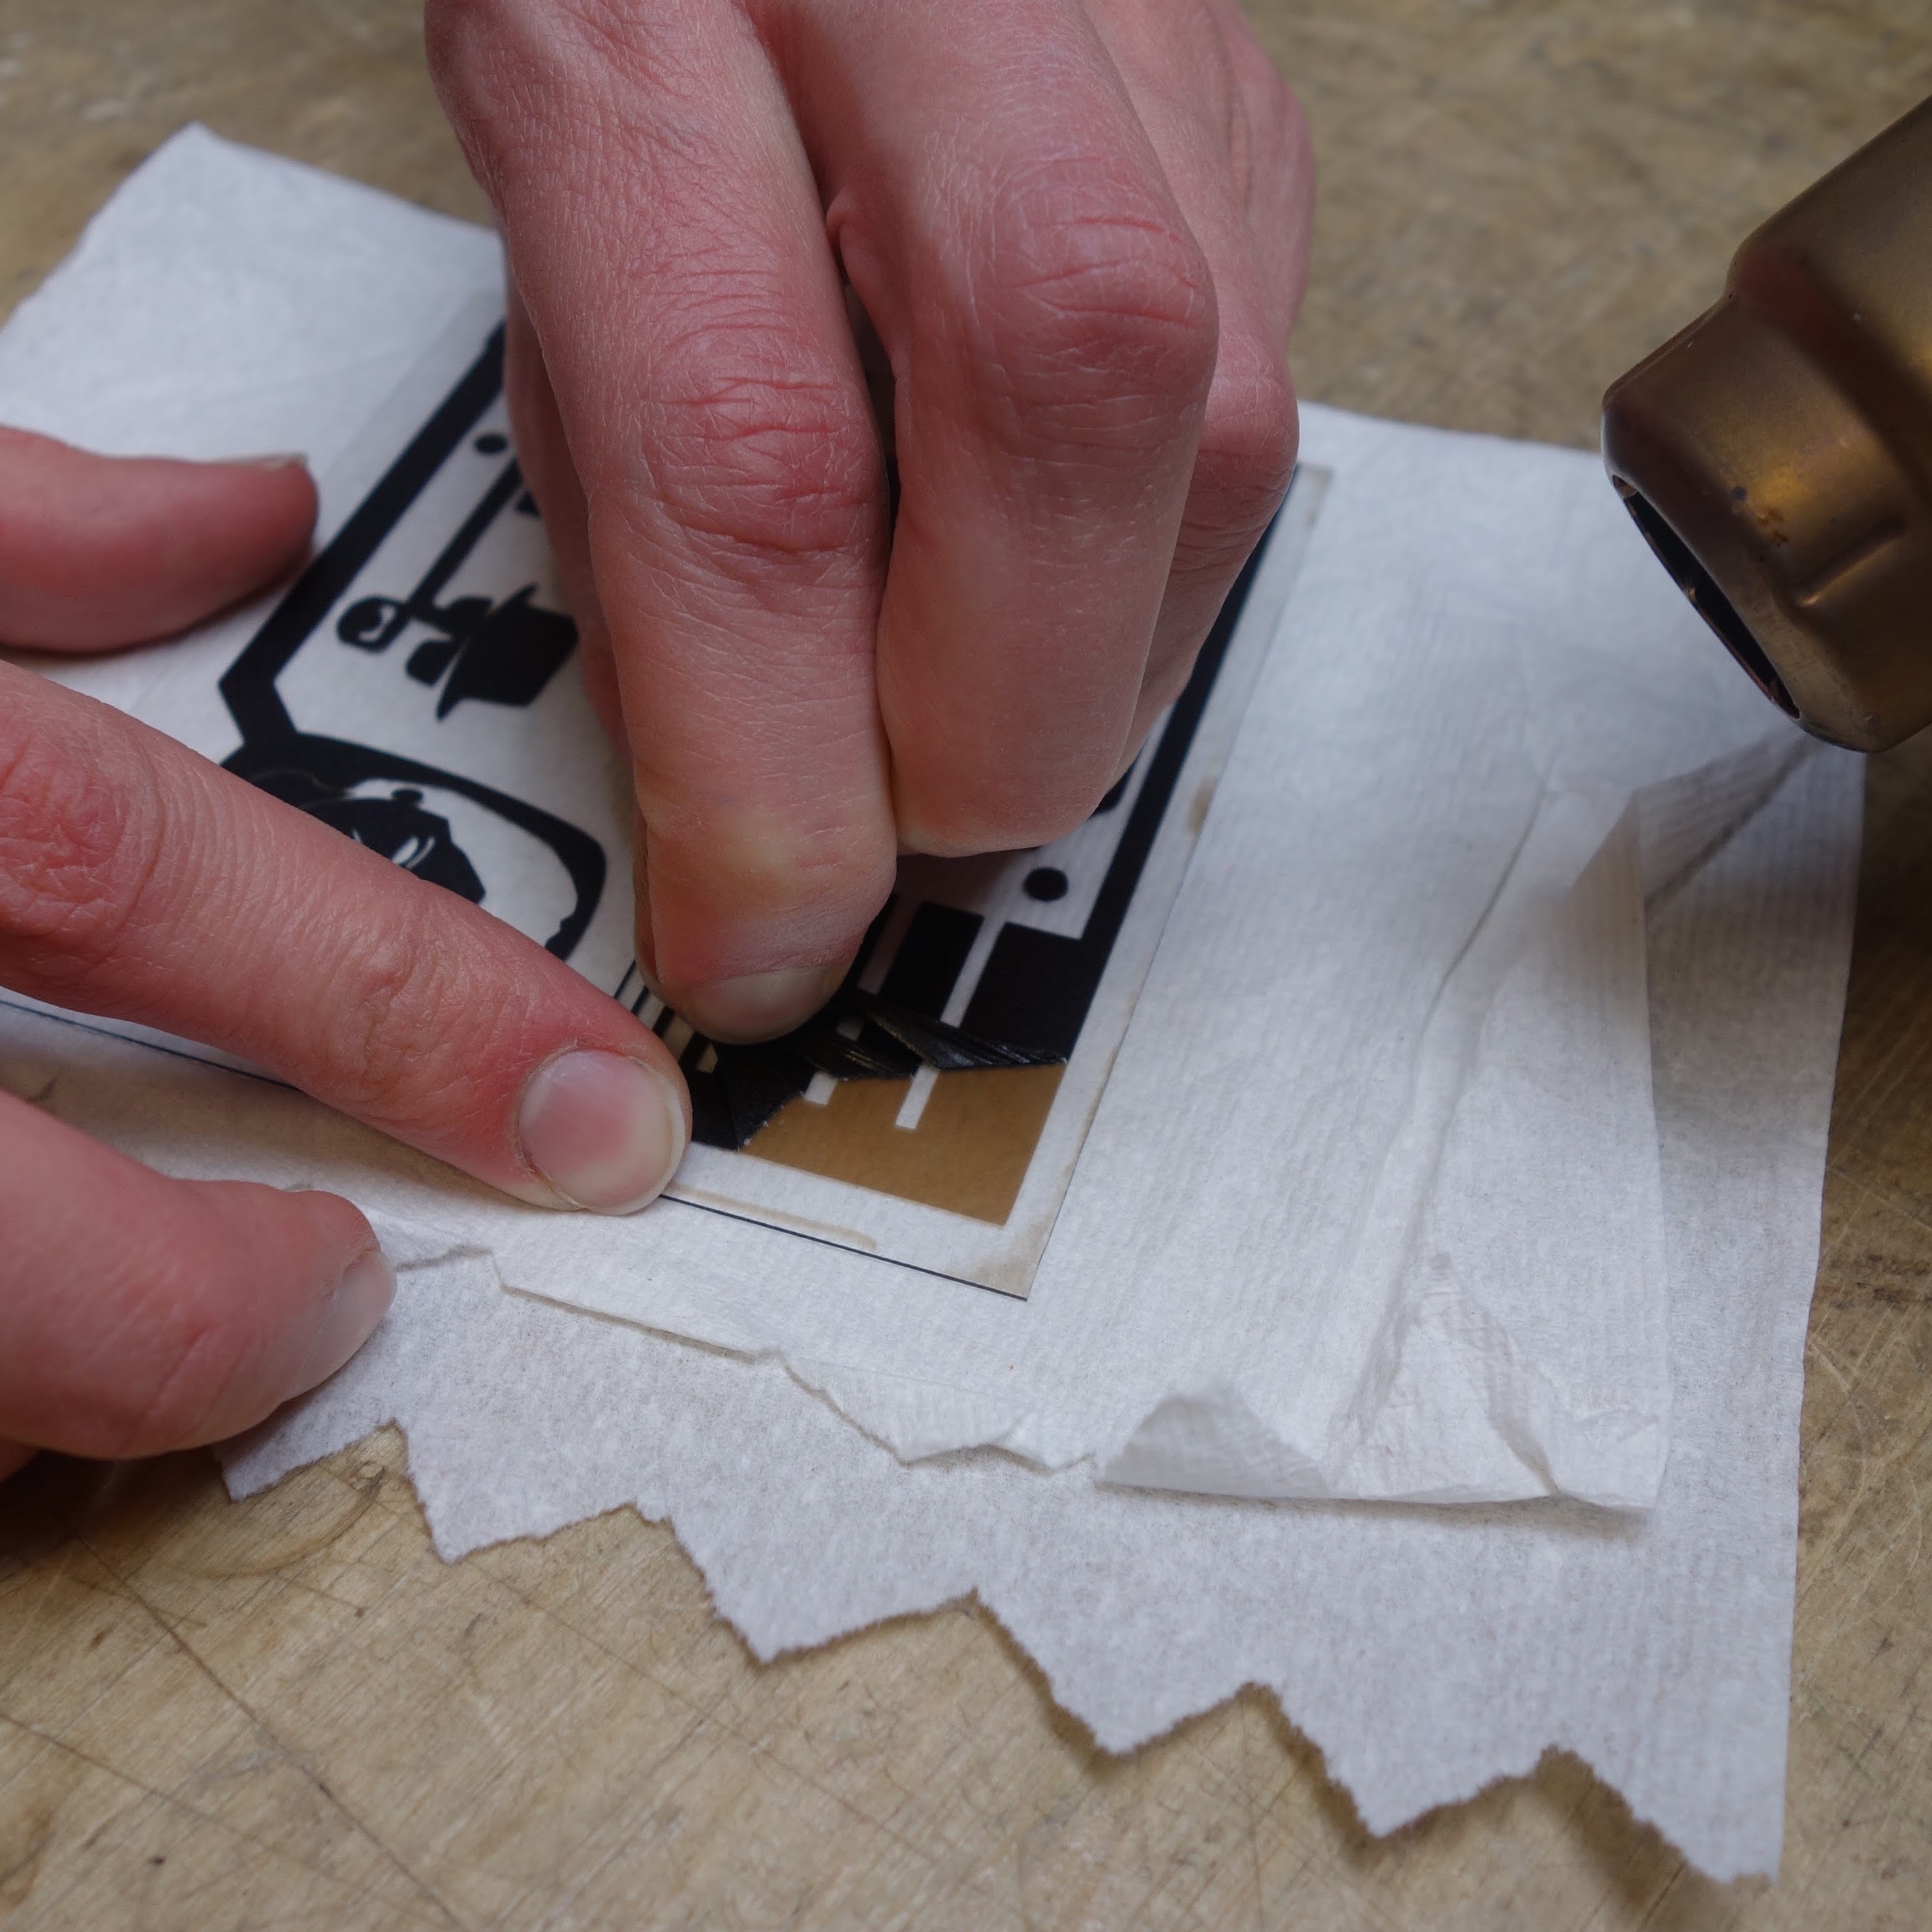
\includegraphics[width=0.22\textwidth]{./Bilder/Schritt2.jpg}
    }
    ~
     \subfigure[Entwickelte Glasscheibe]{
   		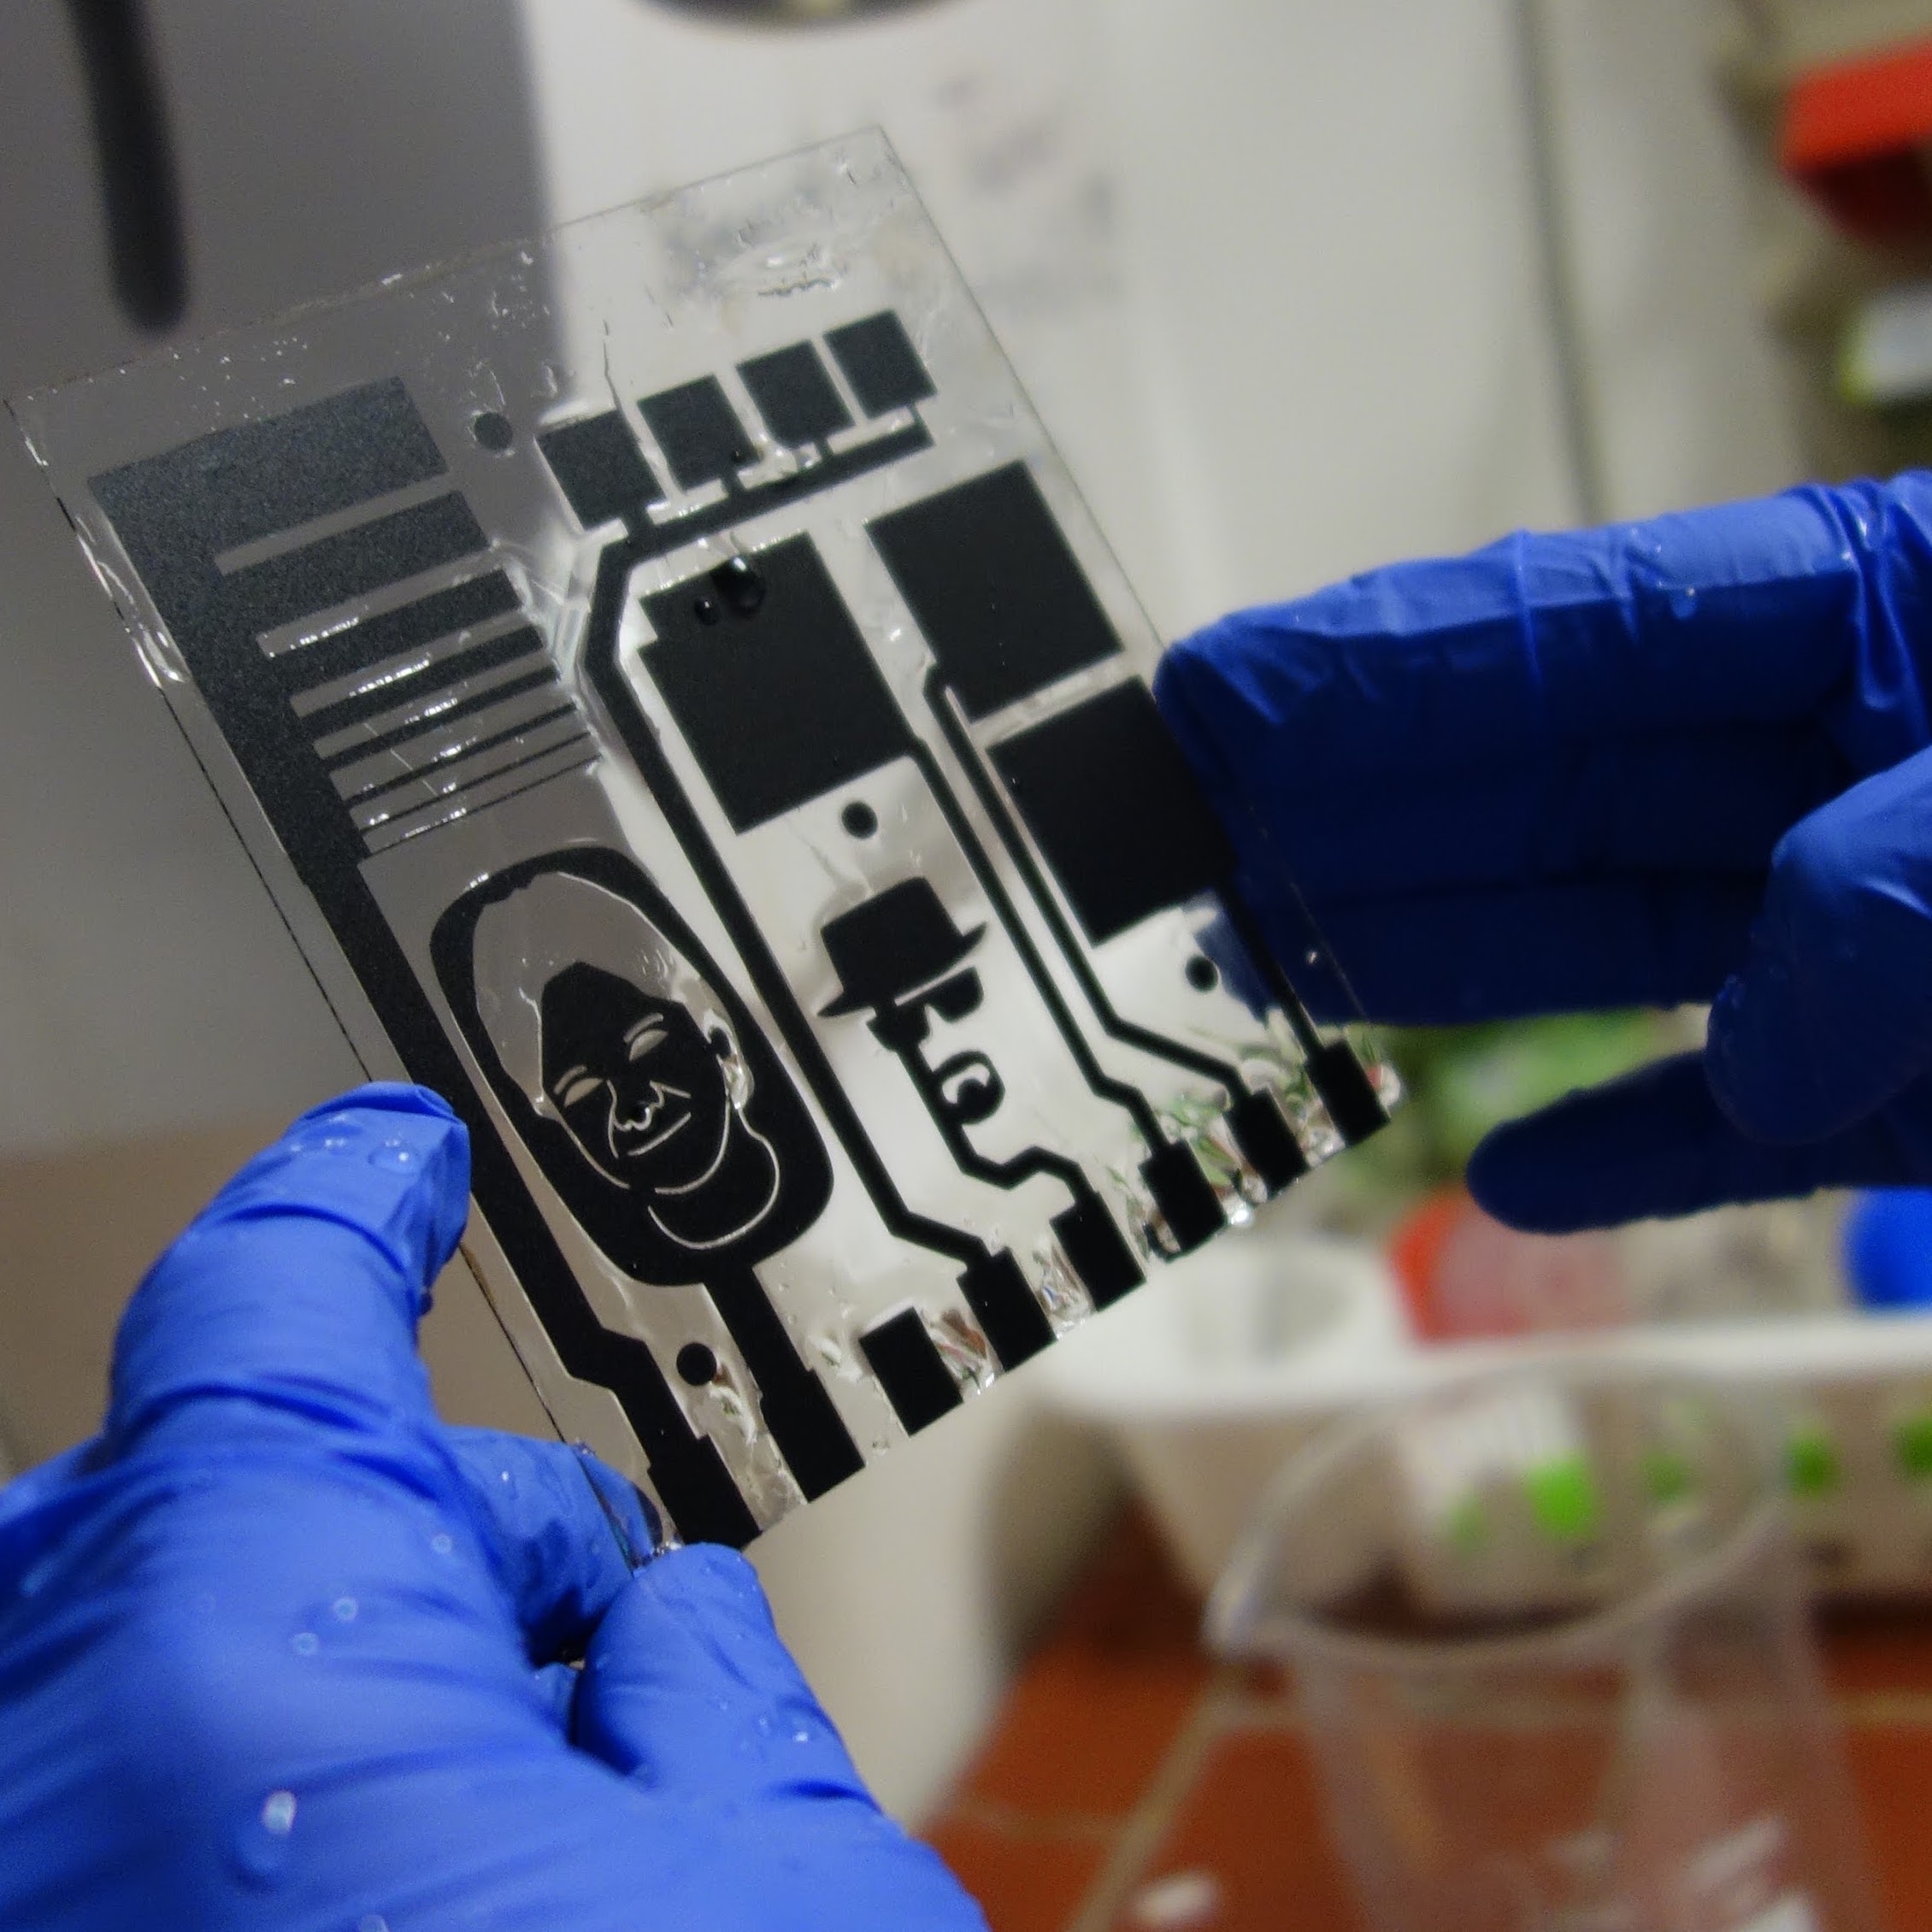
\includegraphics[width=0.22\textwidth]{./Bilder/Schritt3.jpg}
    }
    ~
      \subfigure[Orientierung der Moleküle durch Reiben]{
   		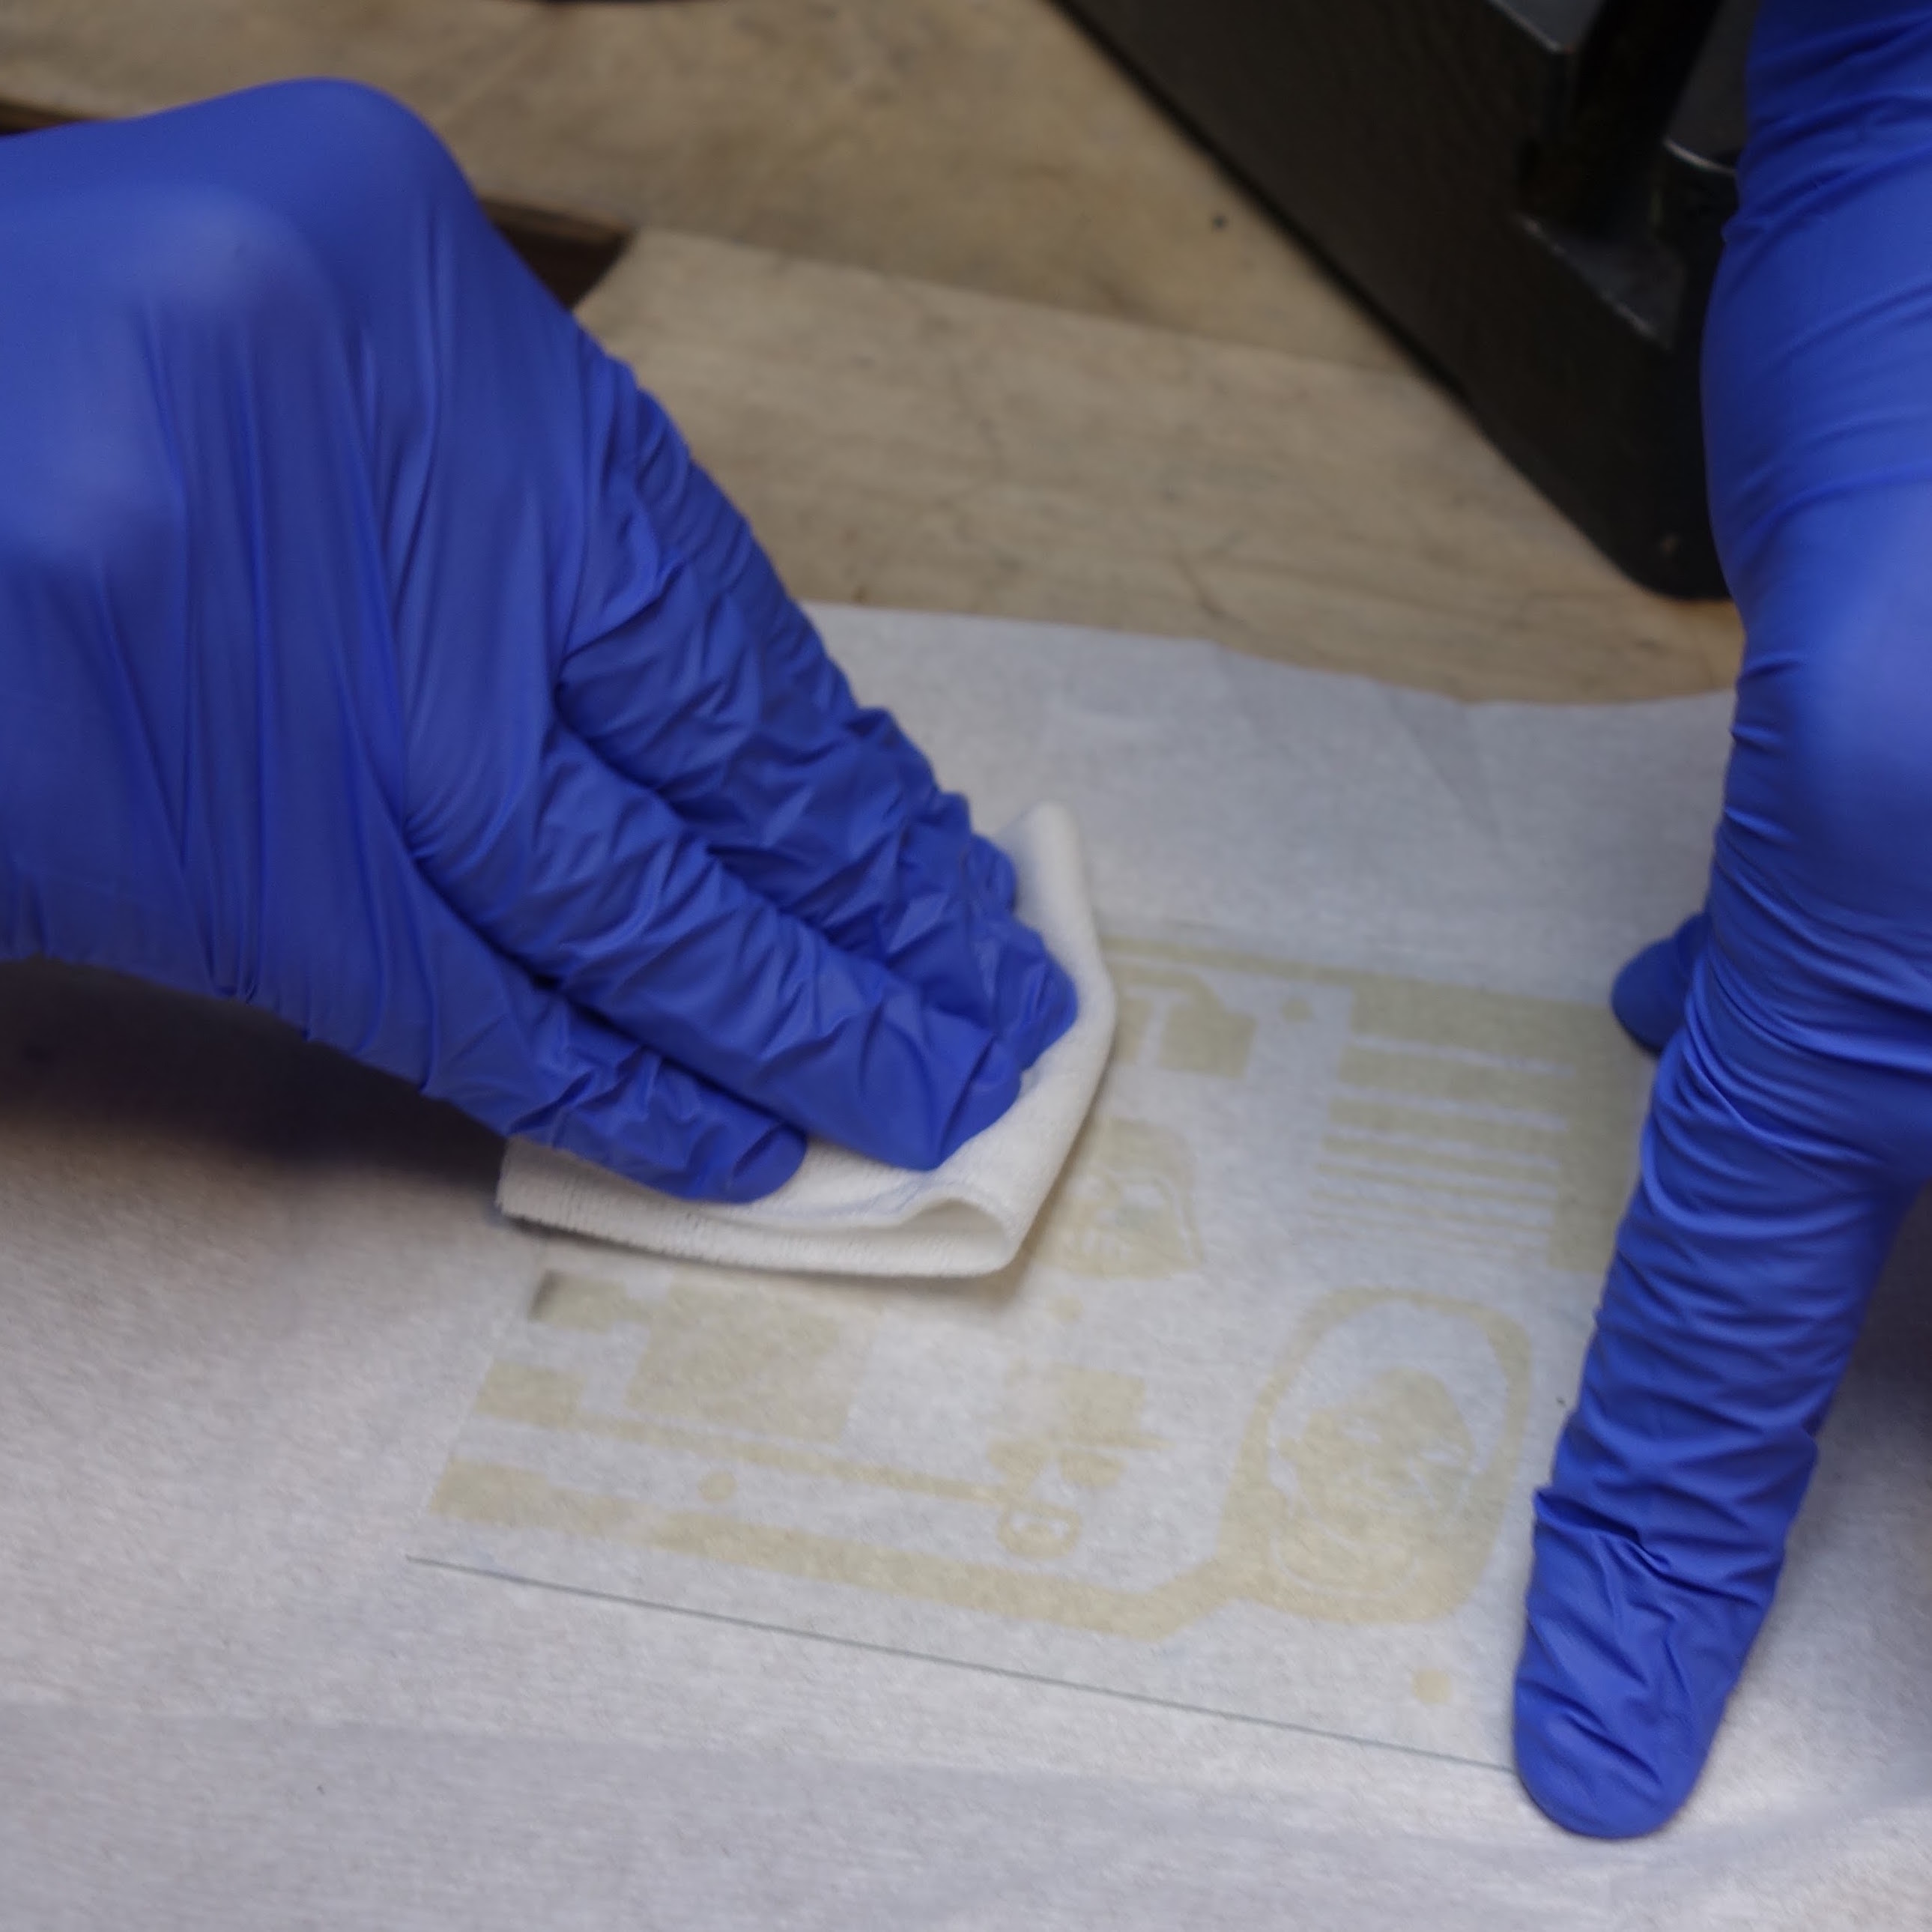
\includegraphics[width=0.22\textwidth]{./Bilder/Reiborientierung.jpg}
    }
    ~
      \subfigure[Kleben des Displays und Einführen des Flüssigkristalls]{
   		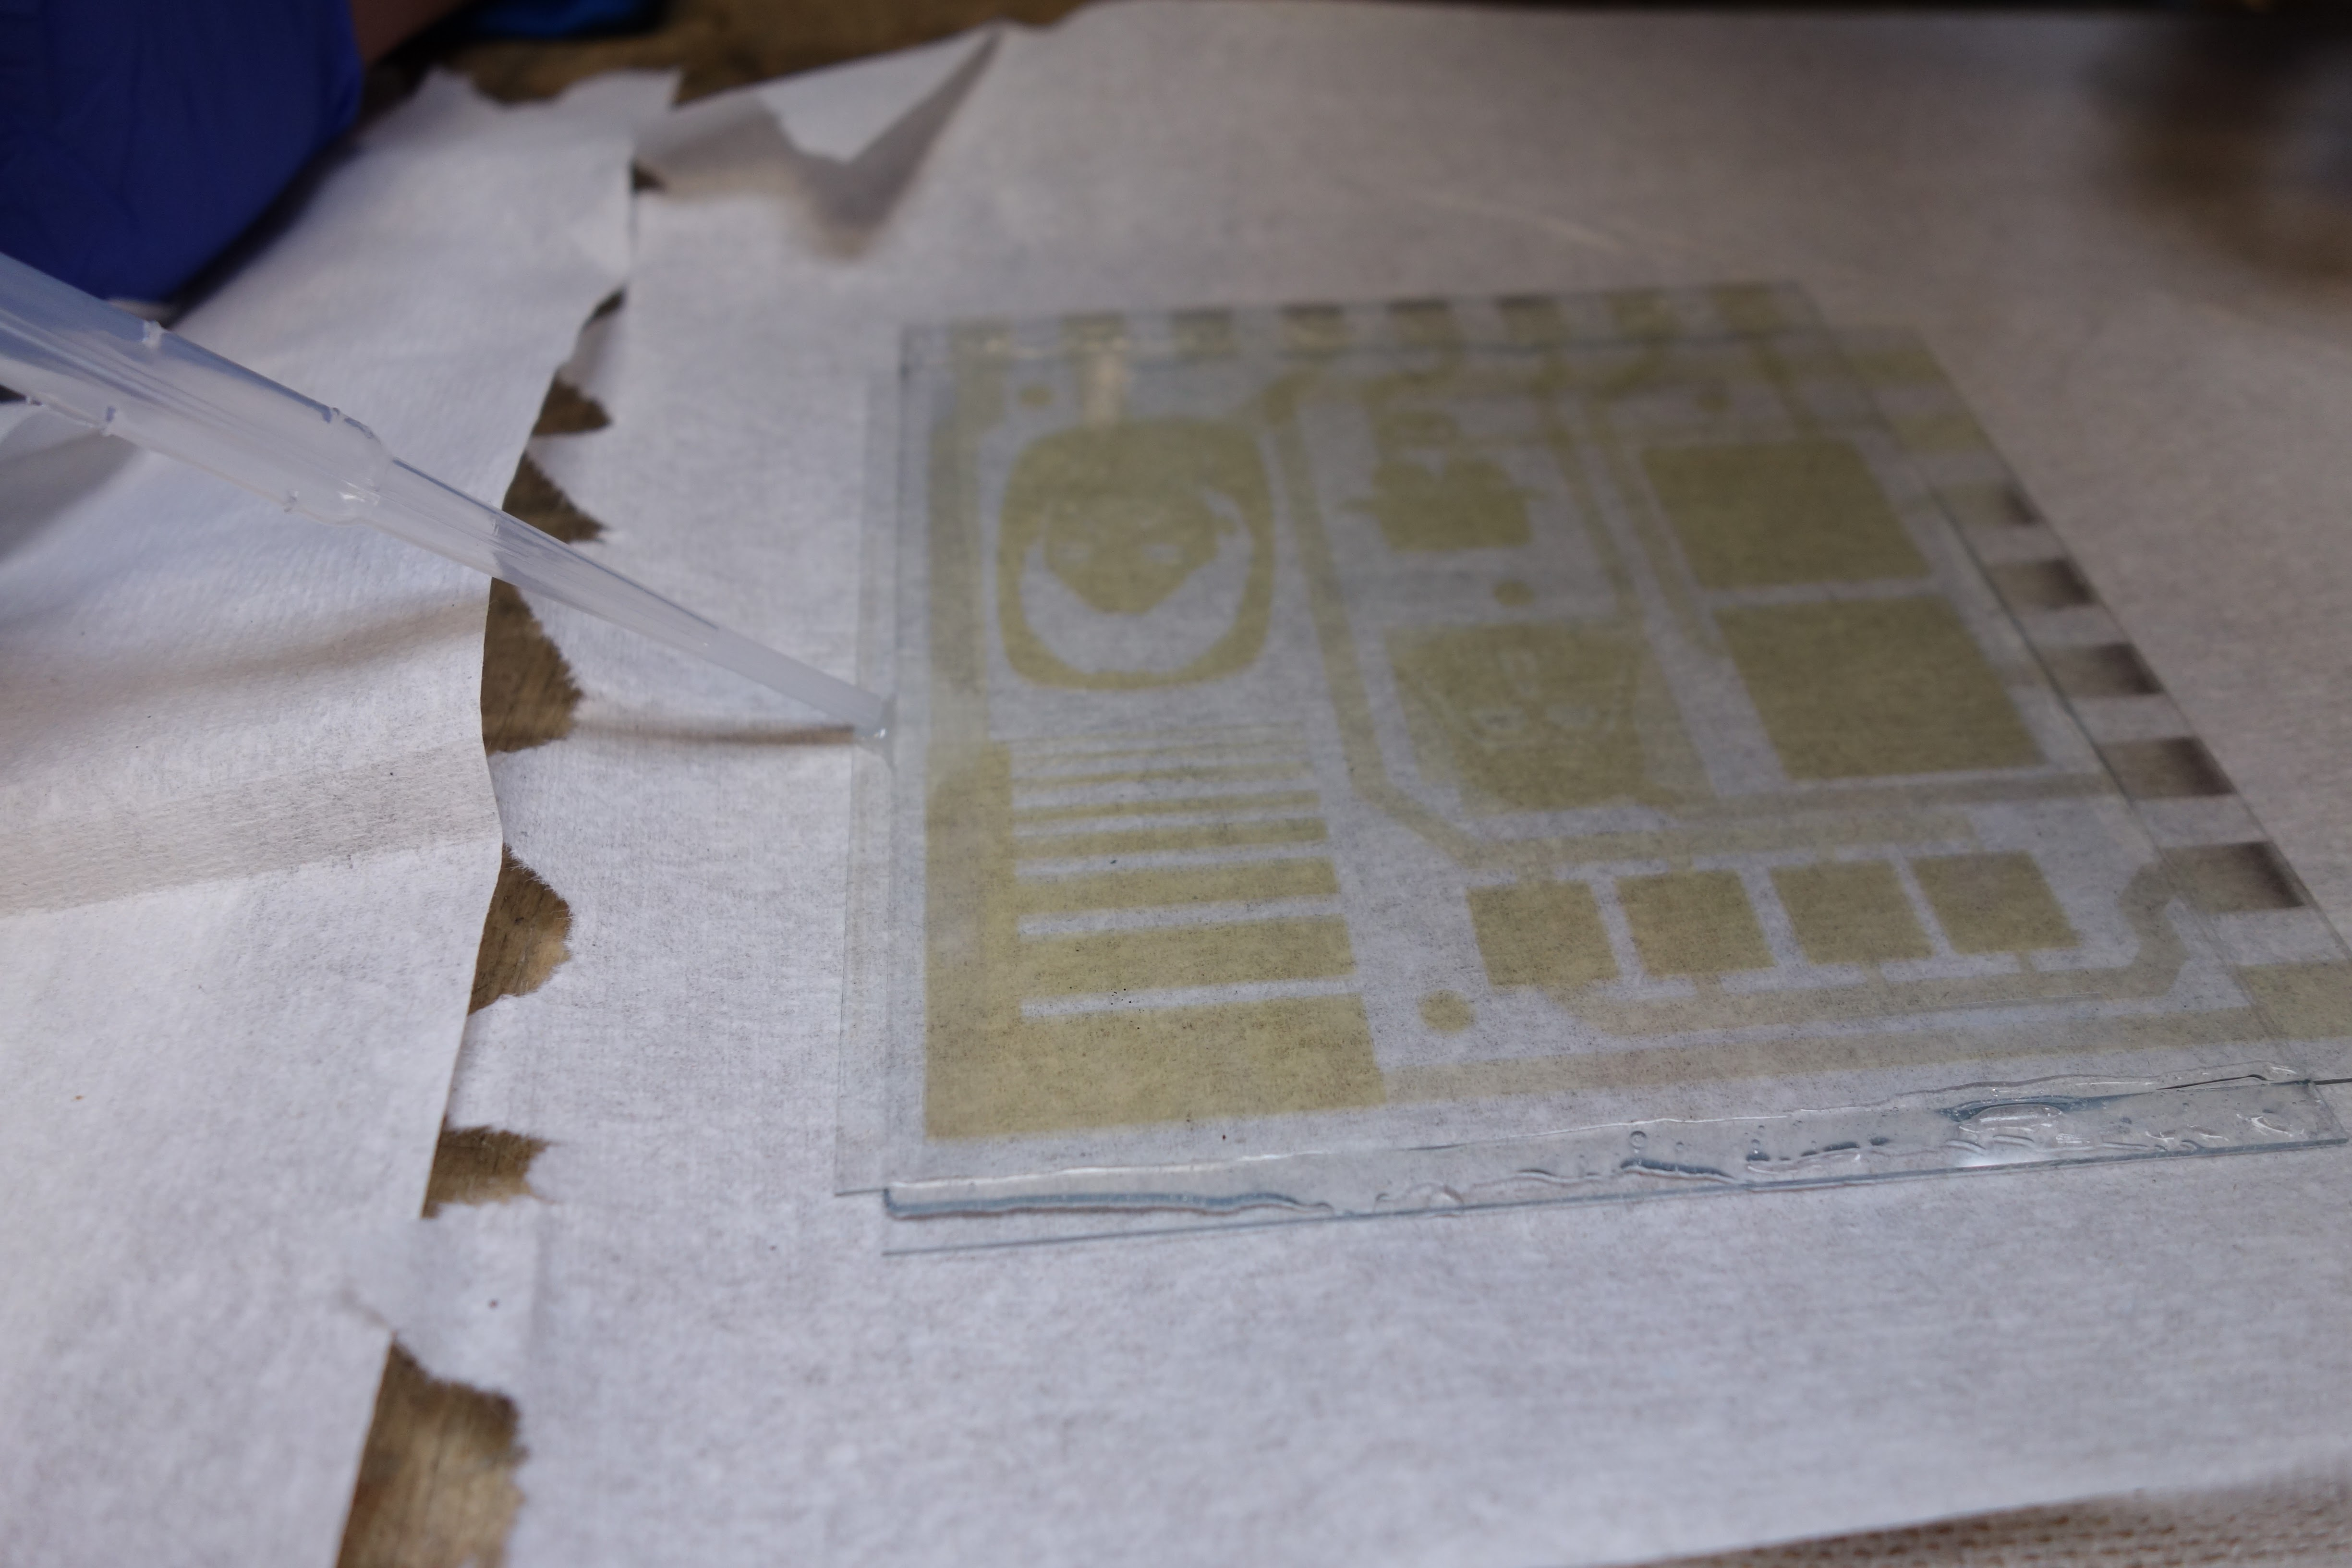
\includegraphics[width=0.22\textwidth]{./Bilder/Fluessigkristall.jpg}
    }
    ~
    \subfigure[Anbringen von Spannung]{
		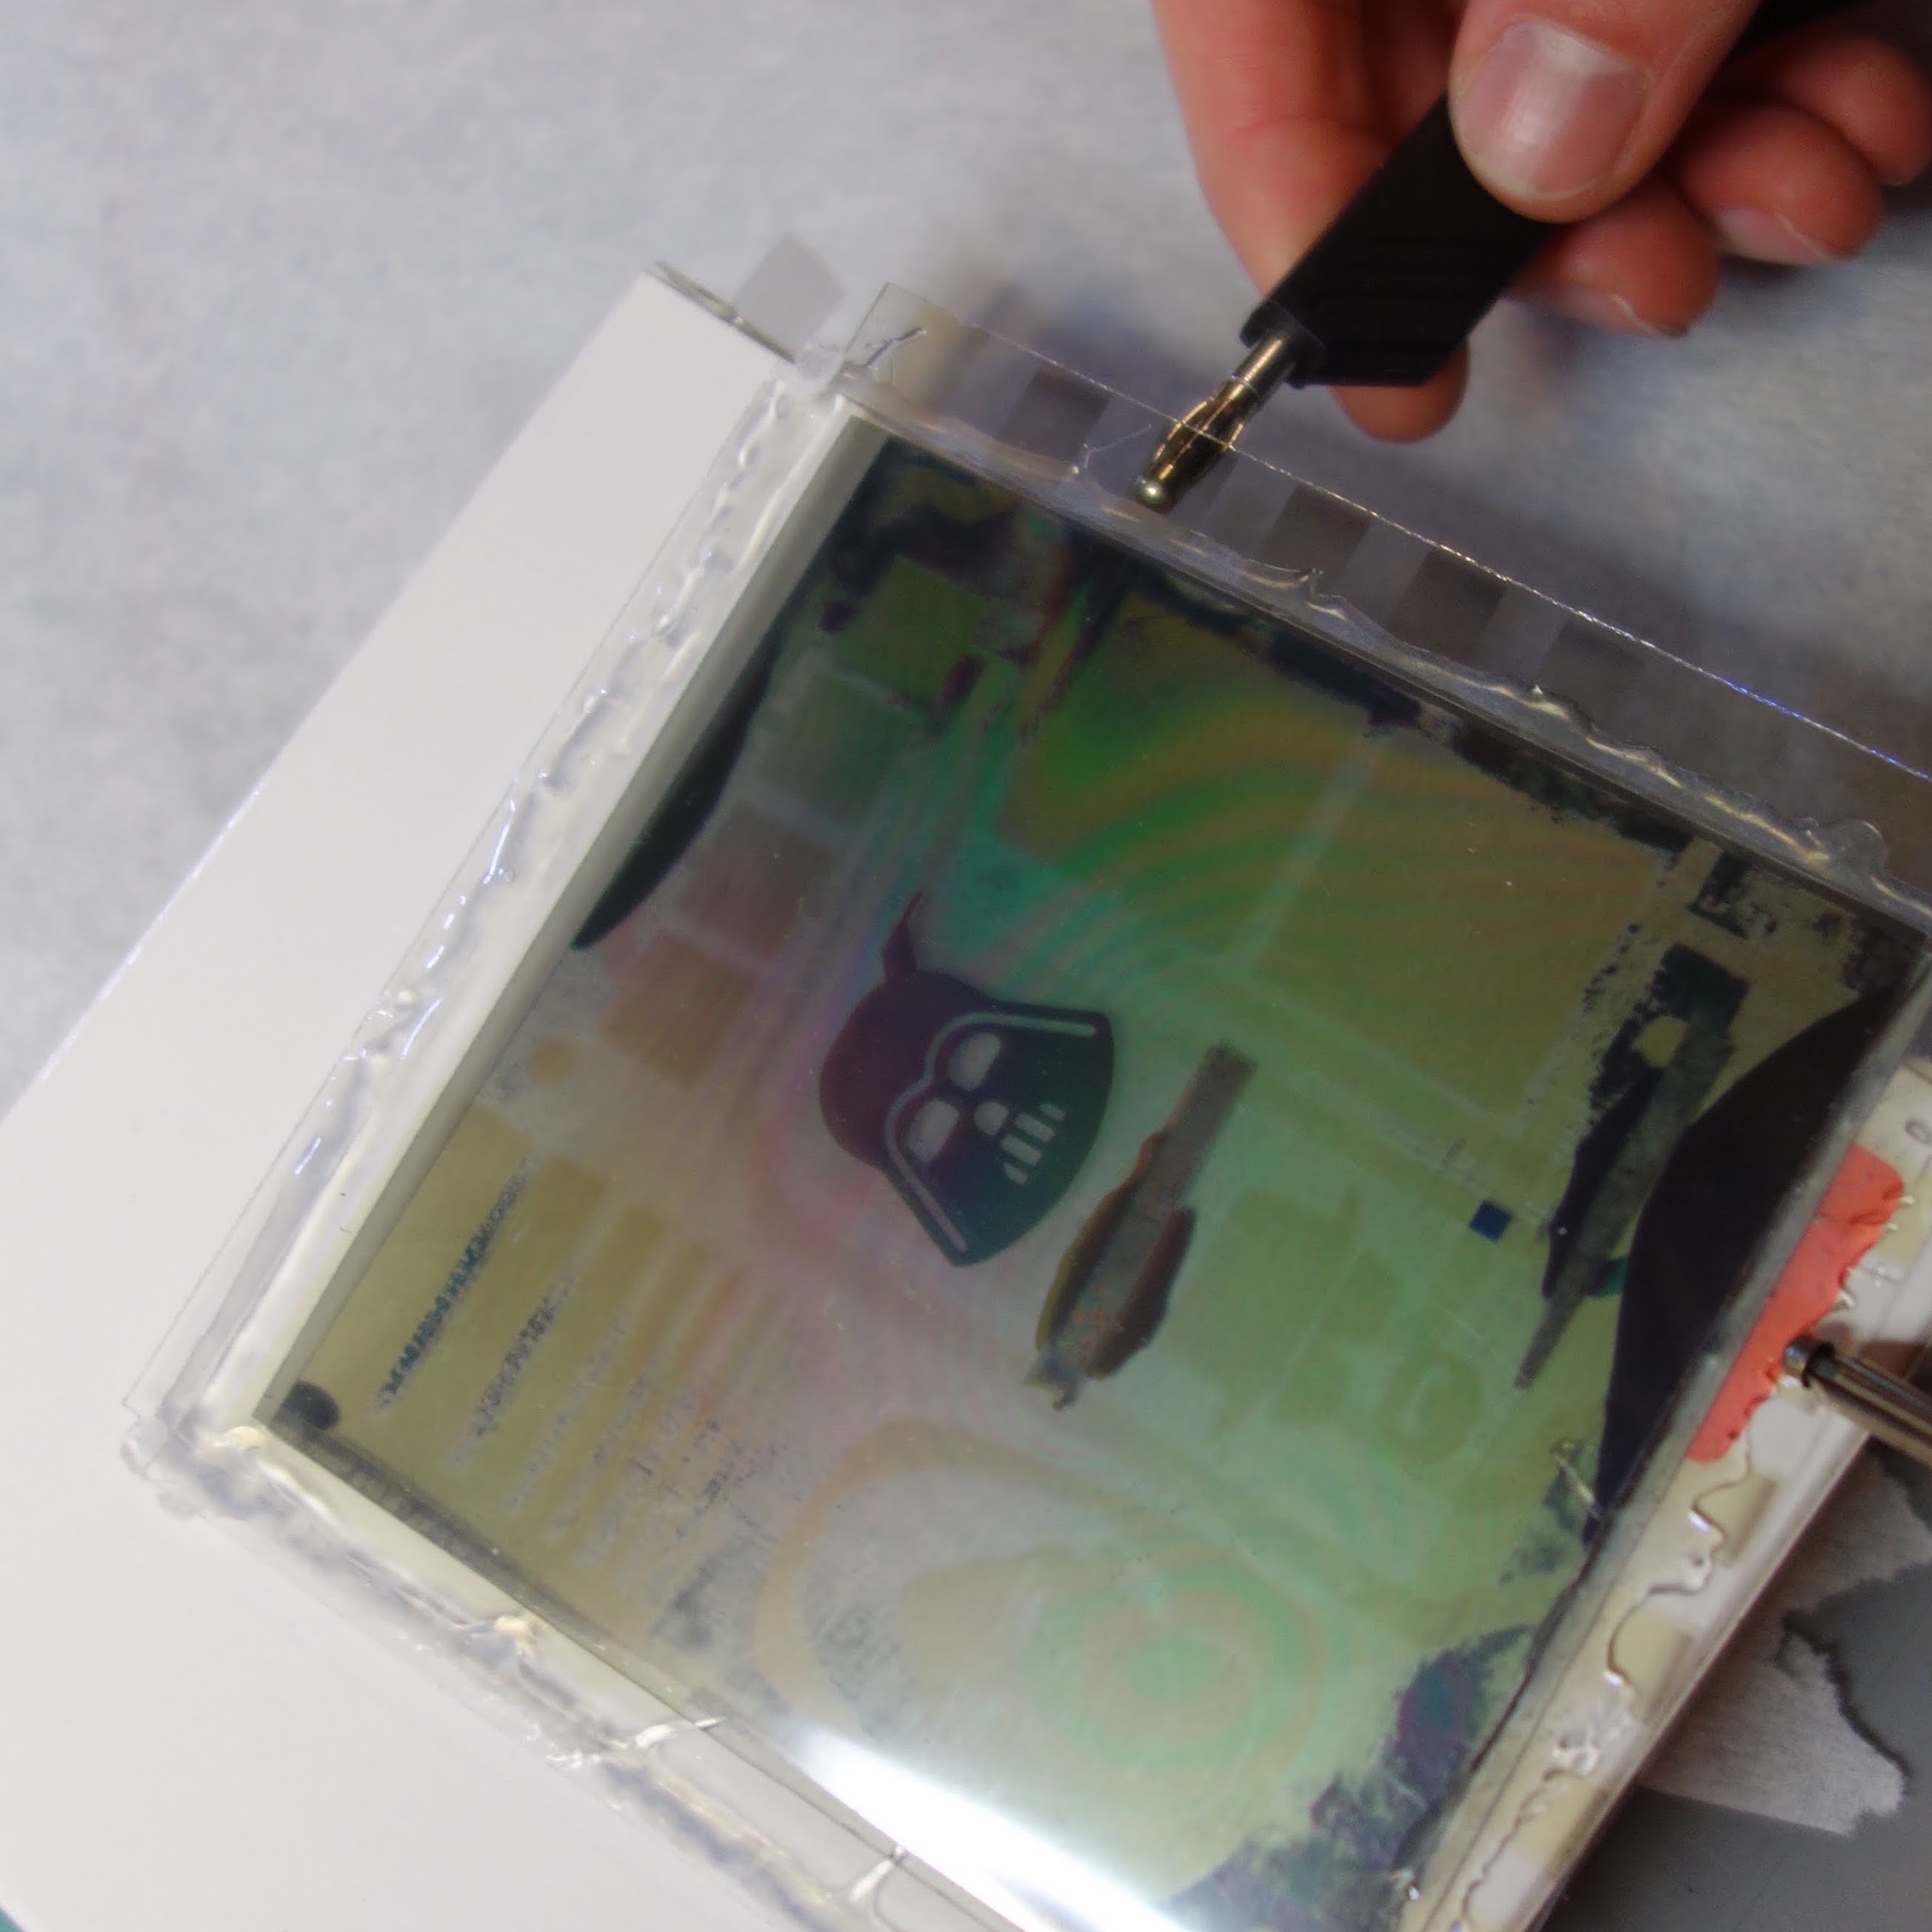
\includegraphics[width=0.22\textwidth]{./Bilder/DarthLeuchtet.jpg}
	}
    \caption{Produktionsschritte bei LCD-Herstellung}
\end{figure}
